\section{Data features and classic methods}
\label{sec:Data features and classic methods}
% 2 pages
To study the feasibility of this project, and to utilise deep learning methods to classify actions from sequential imagery features, videos containing pose-based data, comprehensively reviewing the previous research on data features and feature engineering methods is beneficial to the design of deep models.

%Characteristics of video-based data set
\begin{minipage}[ht]{.48\textwidth}
    \begin{figure}[H]
        \centering
        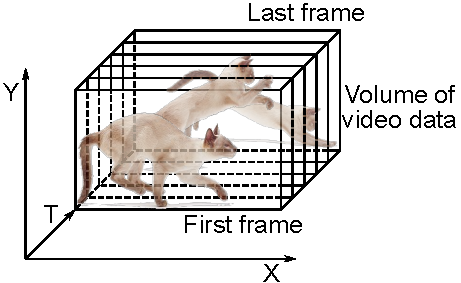
\includegraphics[scale=0.9]{literature/imgs/1-video-volume.pdf}
        \caption{Cubic volume of video data}
        \label{fig:1-video-volume}
    \end{figure}
\end{minipage}
\begin{minipage}[ht]{.5\textwidth}
    \begin{figure}[H]
        \centering
        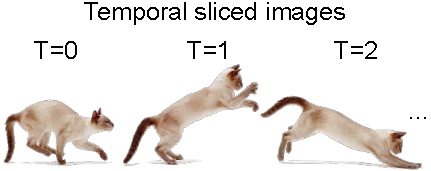
\includegraphics{literature/imgs/2-video-slice.pdf}
        \caption{Slicing the video cube parallel to the X-Y axis}
        \label{fig:2-video-slice}
    \end{figure}
\end{minipage}

Video is composed of a sequence of image data and synchronised audio arranged in the timeline. 
If the audio data beyond the scope of this study is ignored, the 2D images can be stacked along the time axis to form a 3D cube representing the video. Figure \ref{fig:1-video-volume} illustrates an intuitive representation proposed by \citet{fels1999interactive}, which highlights the spatial and temporal characteristics for all videos.
Further, figure \ref{fig:2-video-slice} shows that regular video frames produced by slicing the video cube parallel to the $X-Y$ axis so that computer vision algorithms or deep models for visual tasks can be applied.
As a result, video can be simplified into a series of images to enable applying image processing technology.

%Characteristics of human pose-based features
In each static image containing human pose-based features, what features can be used for posture analysis to classify each image? 
\citet{thrasher2011mood} model the features worthy of attention in human upper body poses and then conduct a pose-based study on mood recognition by analysing and rating the postures of the head, shoulders, trunk, arms in video data.
The data set in their research is closely analogous to the data set in this research because both data sets comprise human facial expressions and upper body poses.

%Link pose-based and video-based features
From posture analysis in a single image to human action recognition in sequential images, it combines pose-based features and video-based data.
For example, \citet{yao2016spatio} propose a paper on spatio-temporal feature extraction with a variety of application scenarios in automatic human activity recognition, such as video information retrieval, intelligent surveillance, and human-computer interaction.
In future research, they point out that deep learning can be a powerful tool for processing these spatio-temporal features and thus will enable the low-level engineered features to fuse with a deep learning framework.

Before deep learning methods are prevalent in the computer vision field, some previous studies have built data sets for the human action recognition task and have conducted studies with classic machine learning methods.

Support vector machines (SVM), a well-known classic machine learning method, has been applied in many researches related to human action recognition.
For example, \citet{schuldt2004recognizing} extract local events such as size, frequency and velocity of moving patterns from videos and create a new video database, KTH data set \footnote{Recognition of human actions: \url{https://www.csc.kth.se/cvap/actions/}}, to evaluate the proposed human actions classification with the SVM method.
Using the SVM method, they carefully model the data representation based on local spatio-temporal features and select appropriate features, kernel tricks, and hyperparameters to obtain the desired results.
%\citet{gorelick2007actions}

Further, \citet{marszalek2009actions} believes that human actions are highly correlated with background scenes, which means the context of the scene can help identify human actions in videos.
They creatively use movie scripts and movie videos, Hollywood-2 data set \footnote{Human Actions and Scenes Dataset: \url{https://www.di.ens.fr/~laptev/actions/hollywood2/}}, to train ``a joint scene-action SVM-based classifier'' with script-to-video alignment.
They explained in detail how to get aligned target actions and target scenes from movies and also used $\mathcal{X}^2$ kernel function in SVM classifier, similar to the research by \citet{schuldt2004recognizing}. In another example, \citet{Soomro2014} focus on action recognition in realistic sports videos.
They conduct research on action localisation and recognition using UCF Sports data set \footnote{UCF Sports Action Data Set: \url{https://www.crcv.ucf.edu/data/UCF_Sports_Action.php}}, including many sports actions collected from television channels.

By reviewing the early research in the human action recognition field, I have introduced the spatio-temporal features in video data sets, the approaches of organising and building the data sets.
Unlike image classification tasks with numerous public data sets available, video data sets are always for individual research questions, so there is no public data set suitable for this research.
As a result, creating a data set is a part of this research, detailed in chapter \ref{chap:Design} and chapter \ref{chap:Implementation}.